\let\negmedspace\undefined
\let\negthickspace\undefined
\documentclass[journal]{IEEEtran}
\usepackage[a5paper, margin=10mm, onecolumn]{geometry}
%\usepackage{lmodern} % Uncomment if needed for pdflatex


\setlength{\headheight}{1cm} % Set the height of the header box
\setlength{\headsep}{0mm}     % Set the distance between the header box and the top of the text

\usepackage{gvv-book}
\usepackage{gvv}
\usepackage{cite}
\usepackage{amsmath,amssymb,amsfonts,amsthm}
\usepackage{algorithmic}
\usepackage{graphicx}
\usepackage{textcomp}
\usepackage{xcolor}
\usepackage{txfonts}
\usepackage{listings}
\usepackage{enumitem}
\usepackage{mathtools}
\usepackage{gensymb}
\usepackage{comment}
\usepackage[breaklinks=true]{hyperref}
\usepackage{tkz-euclide} 
\usepackage{listings}
%\usepackage{gvv}                                        
\def\inputGnumericTable{}                                 
\usepackage[latin1]{inputenc}                                
\usepackage{color}                                            
\usepackage{array}                                            
\usepackage{longtable}                                       
\usepackage{calc}                                             
\usepackage{multirow}                                         
\usepackage{hhline}                                           
\usepackage{ifthen}                                           
\usepackage{lscape}
\usepackage{tikz}
\usepackage{circuitikz}
\usepackage{standalone} % For including external TikZ files

\begin{document}

\bibliographystyle{IEEEtran}
\vspace{3cm}

\title{6.5.1.4}
\author{EE24BTECH11033 - KOLLURU SURAJ}
% \maketitle
% \newpage
% \bigskip
{\let\newpage\relax\maketitle}

\renewcommand{\thefigure}{\theenumi}
\renewcommand{\thetable}{\theenumi}
\setlength{\intextsep}{10pt} % Space between text and floats

\numberwithin{equation}{enumi}
\numberwithin{figure}{enumi}
\renewcommand{\thetable}{\theenumi}
\textbf{Question}:\\
Find the Maximum and Minimum values of the function if exists \\
 \begin{align*}
     y (x) = x^3 + 1
 \end{align*}  
\textbf{Solution : }\\
\textbf{Threotical Solution :}\\

Finding the derivative of the function\\
\begin{align}
    \frac{dy}{dx}=3x^2
\end{align}
We can observe that for any value of $x$ the value of $\frac{dy}{dx}$ is always $\geq$ 0.It is zero at $x=0$.
Which says that the function is increasing that means there is no absolute maximum or minimum\\
\textbf{Computational solution :}\\

Minimum value of the function can be done by \textbf{Gradient decent} method:\\
\textbf{Update the position iteratively}:
\begin{align}
    x_{n+1} = x_{n} - \eta \cdot \frac{dy}{dx}
\end{align}
Taking $x_0$ = 1 as starting point\\
 Here, $\eta = 0.01$, $\eta$ is learning rate.
\begin{align}
    x_{n+1} = x_{n} - \eta \cdot 3x^2
\end{align}
The gradeint descent method stops when $\frac{dy}{dx}= 0$. Because of that the minimum value of the function as computed from gradient descent will be $y\approx 1 , x\approx 0 $

Maximum value of the function can be done by \textbf{Gradient ascent} method:\\
\textbf{Update the position iteratively}:
\begin{align}
    x_{n+1} = x_{n} + \eta \cdot \frac{dy}{dx}
\end{align}
Taking $x_0$ = 1 as starting point\\
 Here, $\eta = 0.01$, $\eta$ is learning rate.
\begin{align}
    x_{n+1} = x_{n} + \eta \cdot 3x^2
\end{align}

This causes $x_n$ to increase indefinitely, because this method stops at x=0 but since we started at x=1 and value of x keeps increasing.


The function increases without bound as $x \rightarrow \infty$ , so \textbf{gradient ascent} will not converge to a maximum. The iteration will continue indefinitely.
so, \textbf{No Maximum exists}\\

\textbf{Computational results :}\\
-Absolute Minimum
\begin{align}
    x \approx 0 , \text{ } y(x) \approx 1
\end{align}
-No Absolute Maximum\\

If we take starting point as x=-1(anything such that $x<0$) we will get minimum as -$\infty$ and maximum as $x \approx 0 , \text{ } y(x) \approx 1$. Because at x=0 $\frac{dy}{dx}=0.$

 \begin{figure}[ht!]
   \centering
   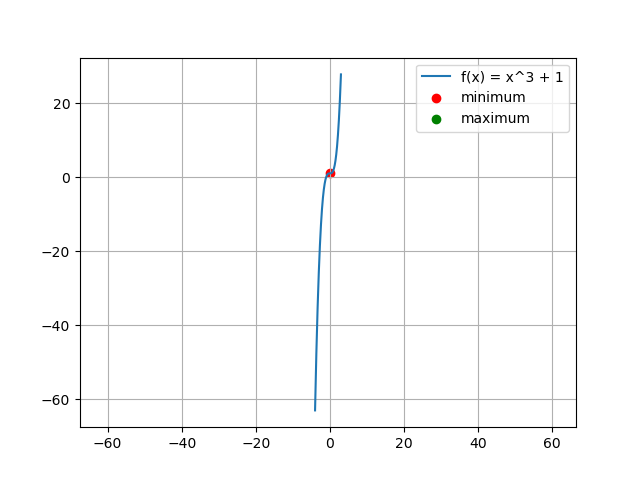
\includegraphics[width=\columnwidth]{figs/Figure_1.png}
\end{figure}
\end{document}
